%%%%%%%%%%%%%%%%%%%%%%%%%%%%%%%%%%%%%%%%%%%%%%%%%%%%%%%%%%%%%%%%%%%%%%%%%%%%%%%%%
%
%  Bachelor's/Master's Thesis       First Name      Last Name       Date
%  "Title"
%  Machine Learning and Data Analytics Lab, FAU Erlangen-Nuernberg
%
%%%%%%%%%%%%%%%%%%%%%%%%%%%%%%%%%%%%%%%%%%%%%%%%%%%%%%%%%%%%%%%%%%%%%%%%%%%%%%%%%
\documentclass{maddoc}
% ++ es werden keine underfull hboxes als Fehler ausgegeben,
%    da das ja nur heißt, dass die Seite noch nicht ganz voll ist
\hbadness=10000

% load the bibliography file
\addbibresource{bibliography.bib}

% Nomenclature
%\usepackage[english]{nomencl}
%\makenomenclature

\usepackage{graphicx}
\usepackage{eurosym}
\usepackage{hhline} % for more flexible horizontal lines in tables
\usepackage{longtable,ltcaption}
\usepackage{minted}
\usepackage{caption}
\usepackage[htt]{hyphenat}
\definecolor{LightGray}{gray}{0.9}

% Ensure that lualatex looks very similar to pdflatex
\setmainfont{texgyretermes}[
  UprightFont = *-regular ,
  BoldFont = *-bold ,
  ItalicFont = *-italic ,
  BoldItalicFont = *-bolditalic ,
  Extension = .otf ,
  Scale = 1.0 ]
\defaultfontfeatures{Ligatures=TeX}

\Titel{Sharing Medical Trial Data in Federated Gaia-X Data Spaces}

\ThesisType{Master's Thesis}
\StudyProgramme{Data Science}

\FirstName{Jan}
\LastName{Šimerda}
\Birthplace{Hradec Králové}
\DateOfBirth{01.08.1999}
\Advisors{Michael~Nissen,~M.~Sc., René~Raab,~M.~Sc., Dr.~med.~Tobias~Steigleder, Prof.~Dr.~Bjoern Eskofier}
\Start{01.03.2024}
\Ende{30.08.2024}
%\PartnerInstitute{Some Other University}

% The date on page iii is automatically set to the current date, but can be overwritten like this:
%\renewcommand{\todayPreamble}{30.05.2022}
% Use this file to define LaTeX macros and placeholders
\newcommand{\OurMethod}{Fancy Name} % example: use \OurMethod as a placeholder for a name that isn't finalized yet.

% define mathematical variables: 
% It's good practice to define variables at one place and add a nomenclature if you have a lot of mathematical variables. 
% This will also help you to keep track of your naming schema.
% Example: 
%\def\states{\vec{x}}           \nomenclature[x]{$\states$}{State vector}

% define chapterabstract
\makeatletter
\newenvironment{chapterabstract}{\hfill\begin{minipage}{\dimexpr\textwidth-0.5cm}}{\end{minipage}\vskip 0.5cm\par\@afterindentfalse\@afterheading}
\makeatother


\pagenumbering{roman}

\begin{document}
\begin{center}
\bfseries
Übersicht
\normalfont
\end{center}

Datenräume sind ein Datenintegrationskonzept, bei dem die Daten nicht in zentralen Datensilos gespeichert werden, sondern an der Quelle gespeichert bleiben.
Einzelne Föderationen werden eingerichtet, um die gemeinsame Nutzung von Daten zu ermöglichen, wobei die Datenkonsumenten über interoperable Standards mit den Datenanbietern verbunden sind.

Gaia-X zielt darauf ab, Datenräume in einer \textit{interoperablen}, \textit{transparenten}, \textit{offenen} und \textit{sicheren} Umgebung zu schaffen, die die \textit{Datenrechte} und die \textit{EU-Vorschriften} respektiert.
Gaia-X Credentials sind ein zentrales Konzept des Ökosystems.
Sie speichern Beschreibungen aller Teilnehmer und logischen Objekte in einer wohldefinierten und überprüfbaren Weise.
Die EU vertraut auf das Projekt, um die Abhängigkeit von ausländischen Tech-Giganten zu verringern und die Innovation in der digitalen Wirtschaft zu fördern.

In der Arbeit wird die Machbarkeit des Austauschs medizinischer Studiendaten in Gaia-X-Datenräumen untersucht.
Die Arbeit umfasst eine Literaturübersicht über Datenräume und verwandte Themen.

Die Hauptmethode der Evaluierung ist die Entwicklung eines Datenaustauschmoduls für die bestehende Plattform zur Speicherung medizinischer Studiendaten---Carecentive---unter Verwendung von Gaia-X-Komponenten und -Spezifikationen.
Das Austauschmodul dient als Proof of Concept und wird später zur Durchführung von Experimenten verwendet, um den Arbeitszustand der Gaia-X-Dienste und -Spezifikationen zu bewerten.
Sechs Experimente wurden entwickelt, um die Funktionalität der Gaia-X Credentials und des Datenaustausch-Workflows zu überprüfen: (1) Erlangung der Konformität für Teilnehmer-Credentials, (2) Erlangung der Konformität für Service-Offering-Credentials, (3) Erlangung der Konformität für Datenprodukt-Credentials, (4) Austausch von Fragebogendaten, (5) Austausch von Withings-Daten, und (6) Datenaustausch mit Verhandlung.

Das Scheitern der Experimente Nr. 2 und 3 deutet auf eine fehlende Implementierung und eine unvollständige Anpassung der implementierten Dienste an die definierten Spezifikationen hin.
Die Unfähigkeit, Experiment Nr. ~6 durchzuführen, zeigt Probleme mit fehlenden Implementierungen von Diensten, die für den Datenaustausch entscheidend sind.
Daher wird der Austausch medizinischer Studiendaten mit Gaia-X in der derzeitigen aktiven Entwicklungsphase als nicht durchführbar angesehen.

\vspace{5.0cm}

\begin{center}
\bfseries
Abstract
\normalfont
\end{center}

Data spaces are a data integration concept in which the data is not stored in central data silos, but the data is kept stored at the source.
Individual federations are set up to enable data sharing, where the data consumers are connected to data providers via interoperable standards.

Gaia-X aims to create data spaces in an \textit{interoperable}, \textit{transparent}, \textit{open}, and \textit{secure} environment that respects \textit{data rights} and \textit{EU regulations}.
Gaia-X Credentials are a central concept of the ecosystem.
They store descriptions of all participants and logical objects in a well-defined and verifiable fashion.
The EU trusts the project to decrease dependence on foreign tech giants and foster innovation in the digital economy.

The work investigates the feasibility of exchanging medical trial data in Gaia-X data spaces.
The thesis includes a literature review on data spaces and related topics.

The main method of evaluation is the development of a data exchange module for the existing platform for storing medical trial data---Carecentive---using Gaia-X components and specifications.
The exchange module acts as a proof of concept and is later used to conduct experiments to assess the working state of the Gaia-X services and specifications.
Six experiments were designed to verify the functionality of Gaia-X Credentials and the data exchange workflow: (1) obtaining compliance for Participant credentials, (2) obtaining compliance for Service Offering credentials, (3) obtaining compliance for Data Product credentials, (4) exchange of questionnaire data, (5) exchange of Withings data, and (6) data exchange with negotiation.

The failure of experiments no.~2 and 3 points to missing implementation and imperfect alignment of implemented services with defined specifications.
The inability to conduct experiment no.~6 demonstrates issues with missing implementations of services crucial for data exchange.
Therefore, the exchange of medical trial data using Gaia-X is deemed unfeasible in the current active development phase.


% Print a table fo contents
\tableofcontents
\cleardoublepage

% Nomenclature
% \addcontentsline{toc}{chapter}{Nomenclature}
%\null\newpage
%\printnomenclature[4em]
%\cleardoublepage

% start arabic page numbers
\pagenumbering{arabic}

% CONTENT
% Here we include the actual content of the thesis.
% Feel free to add/remove/rename the files and include statements according to your needs.
% Each file should start with a \chapter{Title} command


% introduction
%---------------------------------------------------------------
\chapter{Introduction}\label{ch:introduction}

\section{Motivation}\label{sec:motivation}

The ongoing developments of hardware and software in information technology have caused electronic devices to steadily become more compact, lighter,
and more affordable for end customers.
Coupled with advancements in battery life, this trend has enabled the emergence of smart wearable devices,
with the first-ever market-produced ``smartwatches''
\footnote{The \textit{smartness} of the "Pulsar Calculator Watch" though was vastly different from our current
understanding of smart gadgets and was limited to arithmetic calculations.} appearing as early as 1975\cite{ometov_survey_2021}.
Over time, this has ignited a growing interest in these devices among the general public, with now around
30\%\cite{simon_kemp_rise_2023} of internet users owning a smartwatch or a smart wristband.

The hype around consumer-available wearable devices didn't leave the healthcare industry untouched.
Even though digital technologies have been successfully used in clinical for many years, the recent advances in
hardware and analytic capabilities have caused an explosion of interest in the use of digital technologies to
facilitate data collection in clinical trials\cite{clay_impact_2017}.

The use of wearable technology in medical trials can potentially offer numerous benefits compared to the
traditional data collection approach.
These include --- but are not limited to --- longitudinal data measurement, out of clinic use, reduced cost, treatment response monitoring and improved data quality\cite{munos_mobile_2016}.

The deployment of smart wearable devices in clinical trials along with their continuous recording capabilities results in significant increases in data volume\cite{munos_mobile_2016}.
Which may extend the possibilities of using deep learning, where the requirement for the size of a training dataset is increased, to analyze this data.

The increase in generated data volume presents an opportunity to exchange this data with other researchers or institutions, which can further reduce the cost of research.

This thesis examines the feasibility of using a Gaia-X-compliant solution to perform this exchange.
\textit{Gaia-X}\cite{gaiax} is an initiative that emerged in 2019 in the EU and whose goal is to govern how data, digital services and infrastructure are exchanged in a decentralized federated environment.
They do this by publishing specifications, parties must follow in order to participate.
Alongside the specifications, they also provide a reference implementation of the software services needed to run a Gaia-X federation under the project name Gaia-X Federation Services\cite{gxfs}.
This includes mainly the framework facilitating data and software transactions and other useful tools, for example, a credential manager or data exchange logger.

\section{Purpose}\label{sec:purpose}

While the initiative already emerged in 2019, saw a continued increase in the number of members, lighthouse projects and national hubs, and was made publicly available in 2023; there have also been reports of implementation delays, lack of agility, excessive bureaucracy and concerns about the market readiness of Gaia-X\cite{say_gaia-x_2024},~\cite{noauthor_inside_2021},~\cite{eichberger_why_2021}.
The purpose of this thesis is to assess the production-readiness of Gaia-X and to determine the feasibility of exchanging healthcare data via Gaia-X compliant processes.
This is done through the development of a Gaia-X-compliant module for data exchange in an existing framework Carecentive\cite{noauthor_carecentivenet_nodate}.
The exact research questions this thesis seeks to answer are outlined in Table~\ref{tab:research-questions}.

\begin{table}
    \centering
    {\renewcommand{\arraystretch}{1.7}
        \begin{tabular}{ p{4cm}|p{11cm} }
            Research Question 1 & Is it feasible to share healthcare data in Gaia-X Data Spaces?\\
            \hhline{--}
            Research Question 2 & What are the technical challenges in implementing Gaia-X-compliant software?
        \end{tabular}
    }
    \caption{Research Questions}
    \label{tab:research-questions}
\end{table}

\section{Outline}\label{sec:outline}

% TODO: reference the chapters, verify at the end of work
This section concludes the first chapter, which clarifies the motivation, purpose of this thesis, the research questions and finally the outline.
Next up, we provide the fundamentals of federated data and services architectures in Chapter 2.
The next chapter --- Chapter 3 --- then follows up with a deep dive on literature related to the topic of this thesis.
The Chapter 4 serves to clarify the methods of this work used to answer the research questions stated in this chapter.
The Chapter 5 states the results of this work, which are then discussed in Chapter 6.
Lastly, Chapter 7 wraps up this thesis and provides a conclusion.

\clearpage


% GAIA-X
%---------------------------------------------------------------

\chapter{Gaia-X}\label{ch:gaiax}

\begin{chapterabstract}
    In this chapter, we will introduce reader to the initiative \textbf{Gaia-X}.
    We will go over its vision, the means to achieve them, their target organizations and how it may help projects like \textbf{Carecentive}.
\end{chapterabstract}

\section{About Gaia-X}\label{sec:about-gaia-x}

The \textbf{Gaia-X} is the initiative led by the ``Gaia-X Association AISBL'' organization.
The association was registered as an \textit{international non-profit association} \textit{(French: Association Internationale sans but lucratif)} in Belgium in January 2021 and is funded privately.
It was founded by \textit{22} companies and organizations in \textit{January 2021}, but at the time of writing (January 2024), the association has over \textit{350} members from backgrounds like data infrastructure providers, IT startups research institutions and business associations. % TODO: update before completing the thesis
Additionally, representatives from business, politics, academia, research, technology, policy, government, and science from Europe and beyond cooperate with the \textit{Gaia-X Association AISBL} in their mission.
The association claims to have no business interest.~\cite{gaiax}

\section{The Goal}\label{sec:gaia-x-goal}

The goal of the \textbf{Gaia-X} initiative is to enable exchange of data in a \textit{safe} and \textit{trustworthy} environment.
The coveted outcome is a federated system connecting many cloud service providers and users together in an environment that is \textit{interoperable} \textit{transparent}, \textit{open}, \textit{secure}, and respects \textit{data rights} and \textit{EU regulations}.~\cite{gaiax}

\section{The structure}\label{sec:the-structure}

The organisational structure of the ``Gaia-X Association AISBL'' is well-defined and transparent.
The topmost body of the \textit{association} is the \textbf{General Assembly}.
It is composed of all the members of the \textit{association} and has complete authority to carry out the objectives of the \textit{Gaia-X initiative}.~\cite{gaiax}

Under the \textbf{General Assembly} are the boards \em \textit{Governmental Advisory Board}, \textit{General Advisory Board} and the \textit{Board of Directors}.
The \textbf{Board of Directors} is elected by the \textbf{General Assembly} and is headed by a Chairperson and Vice-Chairperson. % TODO: find out how the General Advisory Board and the Governmental Advisory Board are selected
Its purpose is to decide on important matters regarding the \textit{Gaia-X Association}.~\cite{gaiax} % TODO: clarify what the 'important matters' are?

Next up is the \textbf{Management Board} and its chairs \em \textit{Policy Rules Committee}, \textit{Data Spaces Business Committee}, and the \textit{Technical Committee}.
Each of the committees also has its own \textit{Working Group}.
The \textbf{Management Board} is appointed by the \textit{Board of Directors} and is composed of the Chief Executive Officer (CEO), the Chief Operating Officer (COO), the Chief Technical Officer (CTO), the Digital Communications Director and the Head of Finance and Administration.
Its purpose is the management of daily activities of \textit{Gaia-X Association}.~\cite{gaiax}

\begin{figure}
    \centering
    \includegraphics[width=\textwidth]{assets/management-board-structure}
    \caption{~Organisational structure of the Gaia-X Association~\cite{gaiax}}\label{fig:organisational-board-structure}
\end{figure}

\subsection{Data Spaces Business Committee}\label{subsec:data-spaces-business-committee}

The \textit{Data Spaces Business Committee (DSBC)} focuses on collecting \textit{economic}, \textit{functional}, \textit{operational} and \textit{legal} requirements that facilitate seamless collaboration and interconnection between \textit{Data Spaces}, \textit{Ecosystems}, \textit{Lighthouse Projects} and respective \textit{Hubs}. % FIXME: Data Spaces, Ecosystems, Lighthouse Projects and Hubs not defined yet
Furthermore, the \textit{DSBC} supports the creation of Data Spaces by third parties across Europe and beyond.~\cite{gaiax}

\subsection{Policy Rules Committee}\label{subsec:policy-rules-committee}

The \textit{Policy Rules Committee (PRC)} exists to translate the guiding principles of the Gaia-X initiative (\textit{transparency}, \textit{data protection}, \textit{cyber-security}, \textit{portability}, \textit{openness},~\ldots) into High-Level Objectives and to preserve the added value of the \textit{Gaia-X ecosystem}.
The additional role of the \textit{PRC} is to monitor, integrate and define the relationship with EU regulations and external standards.
The Committee guides and delivers the \textit{Gaia-X Trust Framework}, \textit{Gaia-X Policy Rules and Labelling Document} (formerly Policy Rules Document and Gaia-X Labelling Criteria).
These deliverables are provided by the Committee's three \textit{Working Groups} (WG).~\cite{gaiax}
\begin{itemize}
    \item \textbf{Labels \& Qualification} WG:~provides the \textit{Gaia-X Labelling Framework} and prepares the ``Gaia-X Policy Rules and Labelling Document'' together with the \textit{Policy Rules Document} WG
    \item \textbf{Policy Rules Document} WG:~defines \textit{High-Level Objectives} and prepares the ``Gaia-X Policy Rules and Labelling Document'' together with the \textit{Policy Rules Document} WG
    \item \textbf{Compliance} WG:~provides the \textit{Gaia-X Trust Framework}, representing the reference document for the Gaia-X compliance, providing the compulsory set of rules of the Gaia-X Ecosystem
\end{itemize}

\subsection{Technical Committee}\label{subsec:technical-committee}

The purpose of the \textit{Technical Committee (TC)} is to define and implement the technological vision of the \textit{Gaia-X initiative}.
It is in charge of transforming the high-level objectives of Gaia-X and requirements collected from other Committees and Gaia-X members into the \textit{technology roadmap} and is accountable for its contributors.
The Committee drafts and delivers the Gaia-X \textit{Architecture Document}, \textit{technical specifications} and related \textit{reference implementation}.
These deliverables are provided by the Committee's two \textit{Working Groups} (WG).~\cite{gaiax}
\begin{itemize}
    \item \textbf{Architecture} WG:~drafts the ``Gaia-X Architecture Document'', which describes the founding concepts of the \textit{Gaia-X Ecosystem}
    \item \textbf{Service Characteristics} WG:~specifies the Schema for the Self-Descriptions of Providers, their Service Offerings, and the Resources they are composed of
\end{itemize}

\begin{figure}
    \centering
    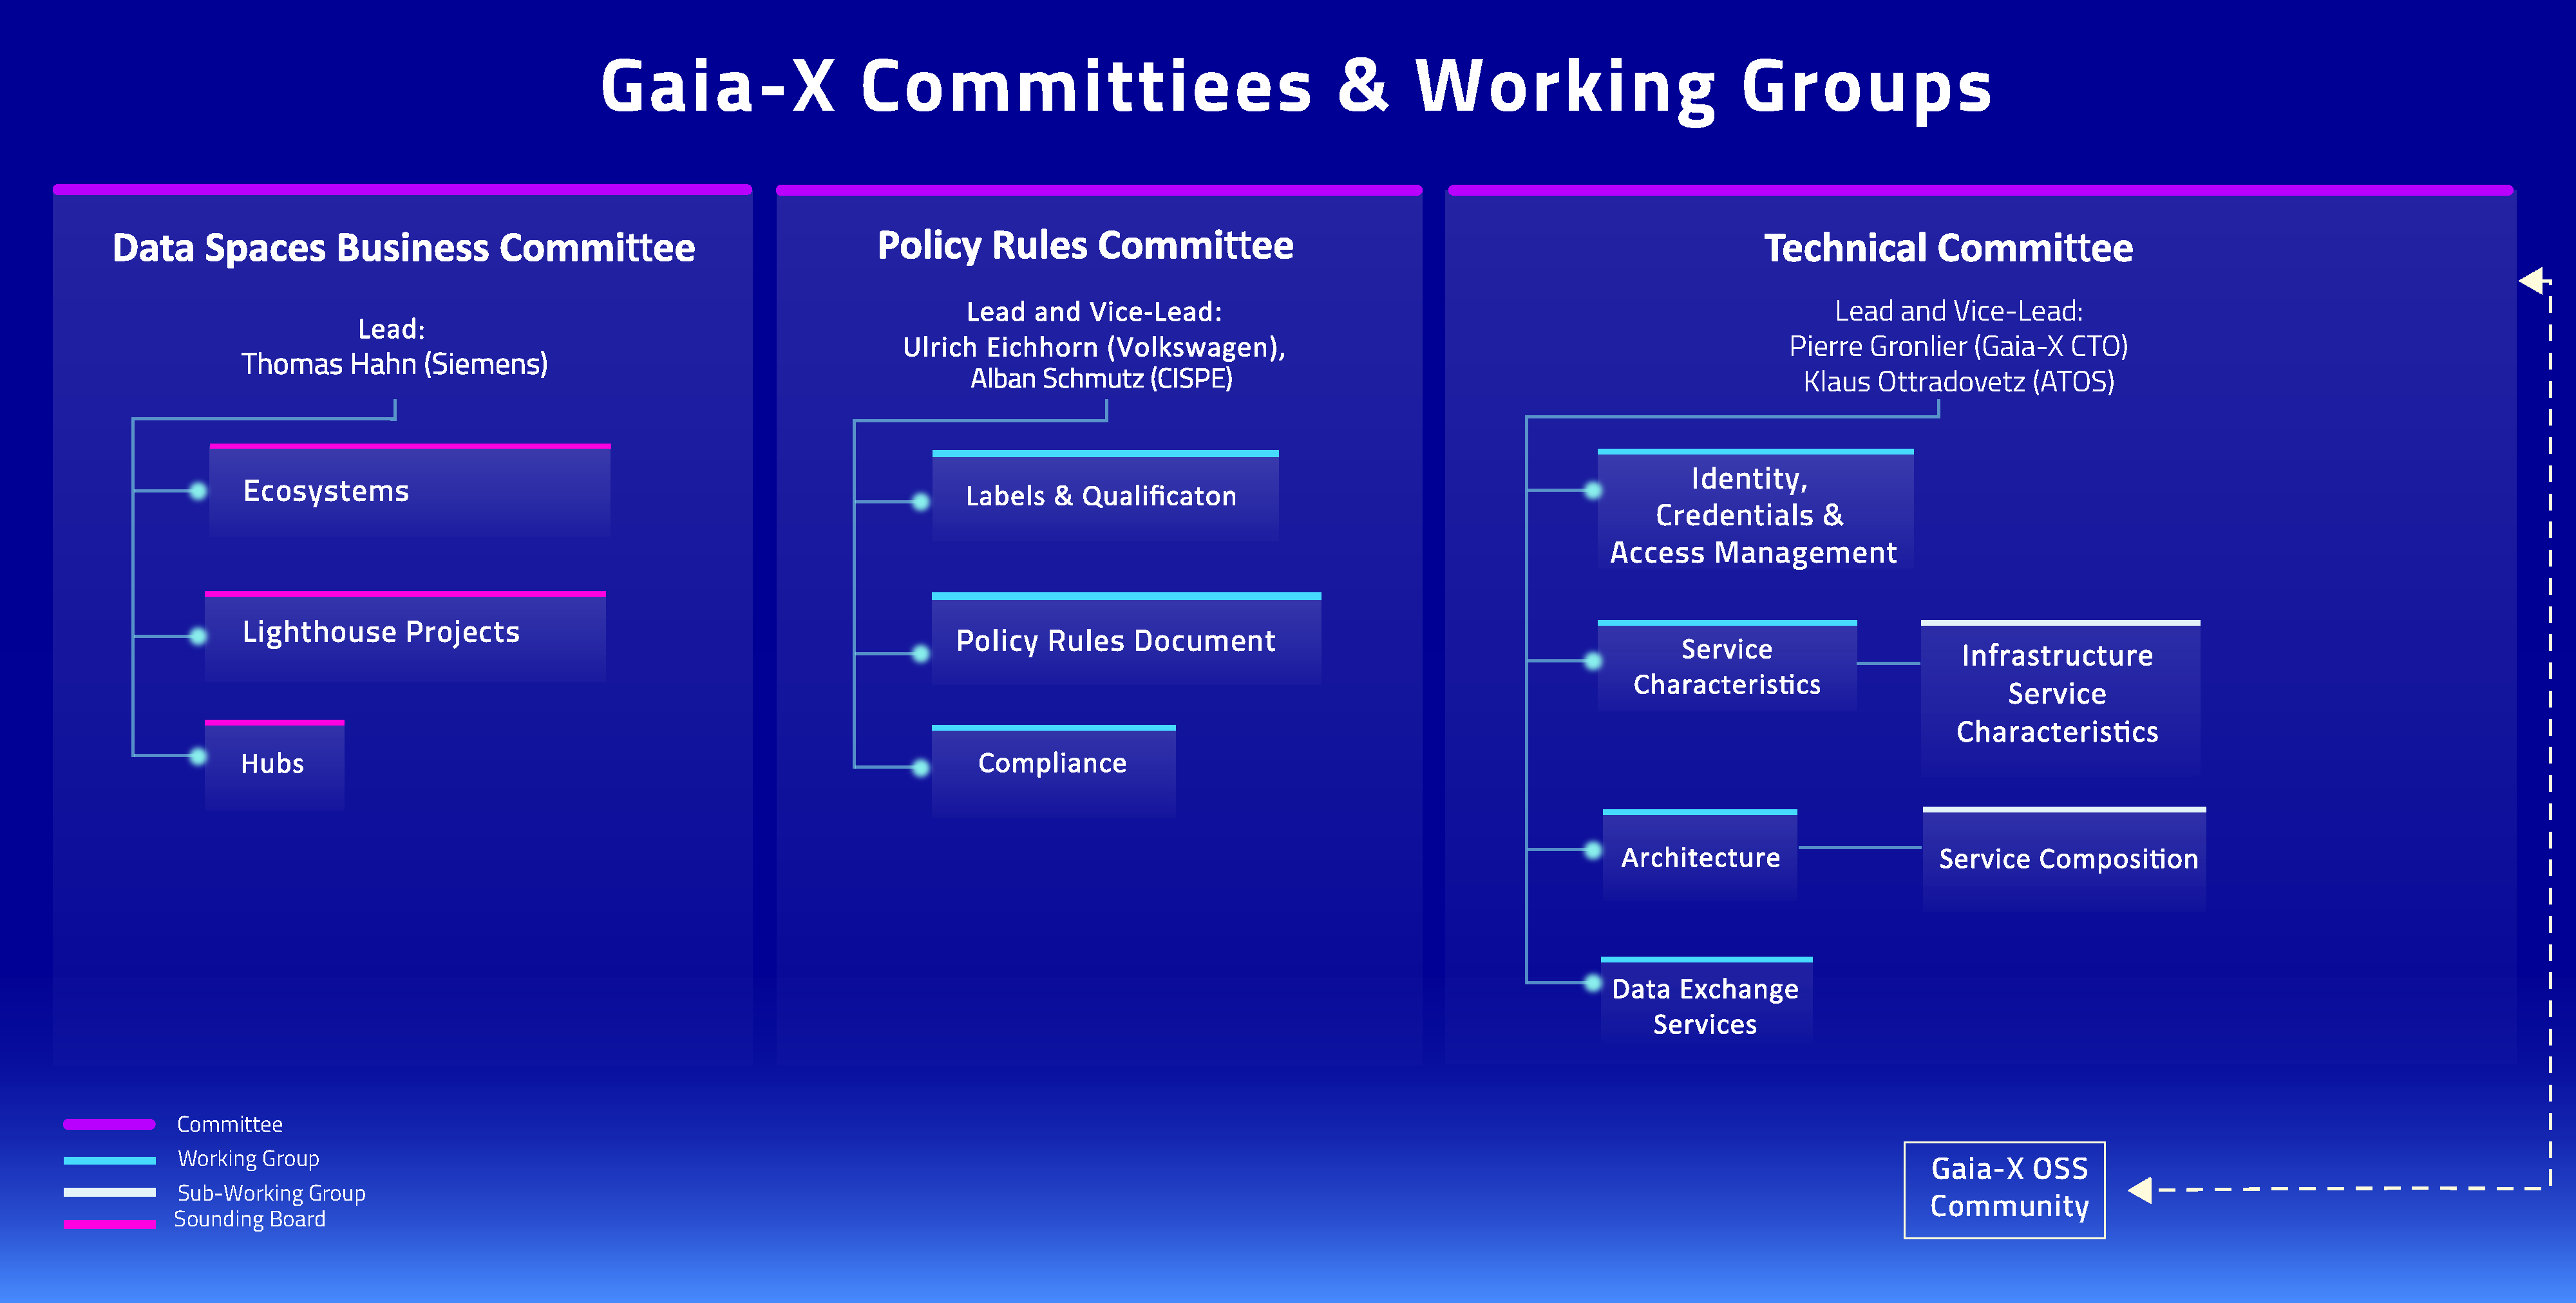
\includegraphics[width=\textwidth]{assets/committees-and-working-groups}
    \caption{~Organisational structure Committees and their Working Groups~\cite{gaiax}}\label{fig:organisational-committees-structure}
\end{figure}

\begin{figure}
    \centering
    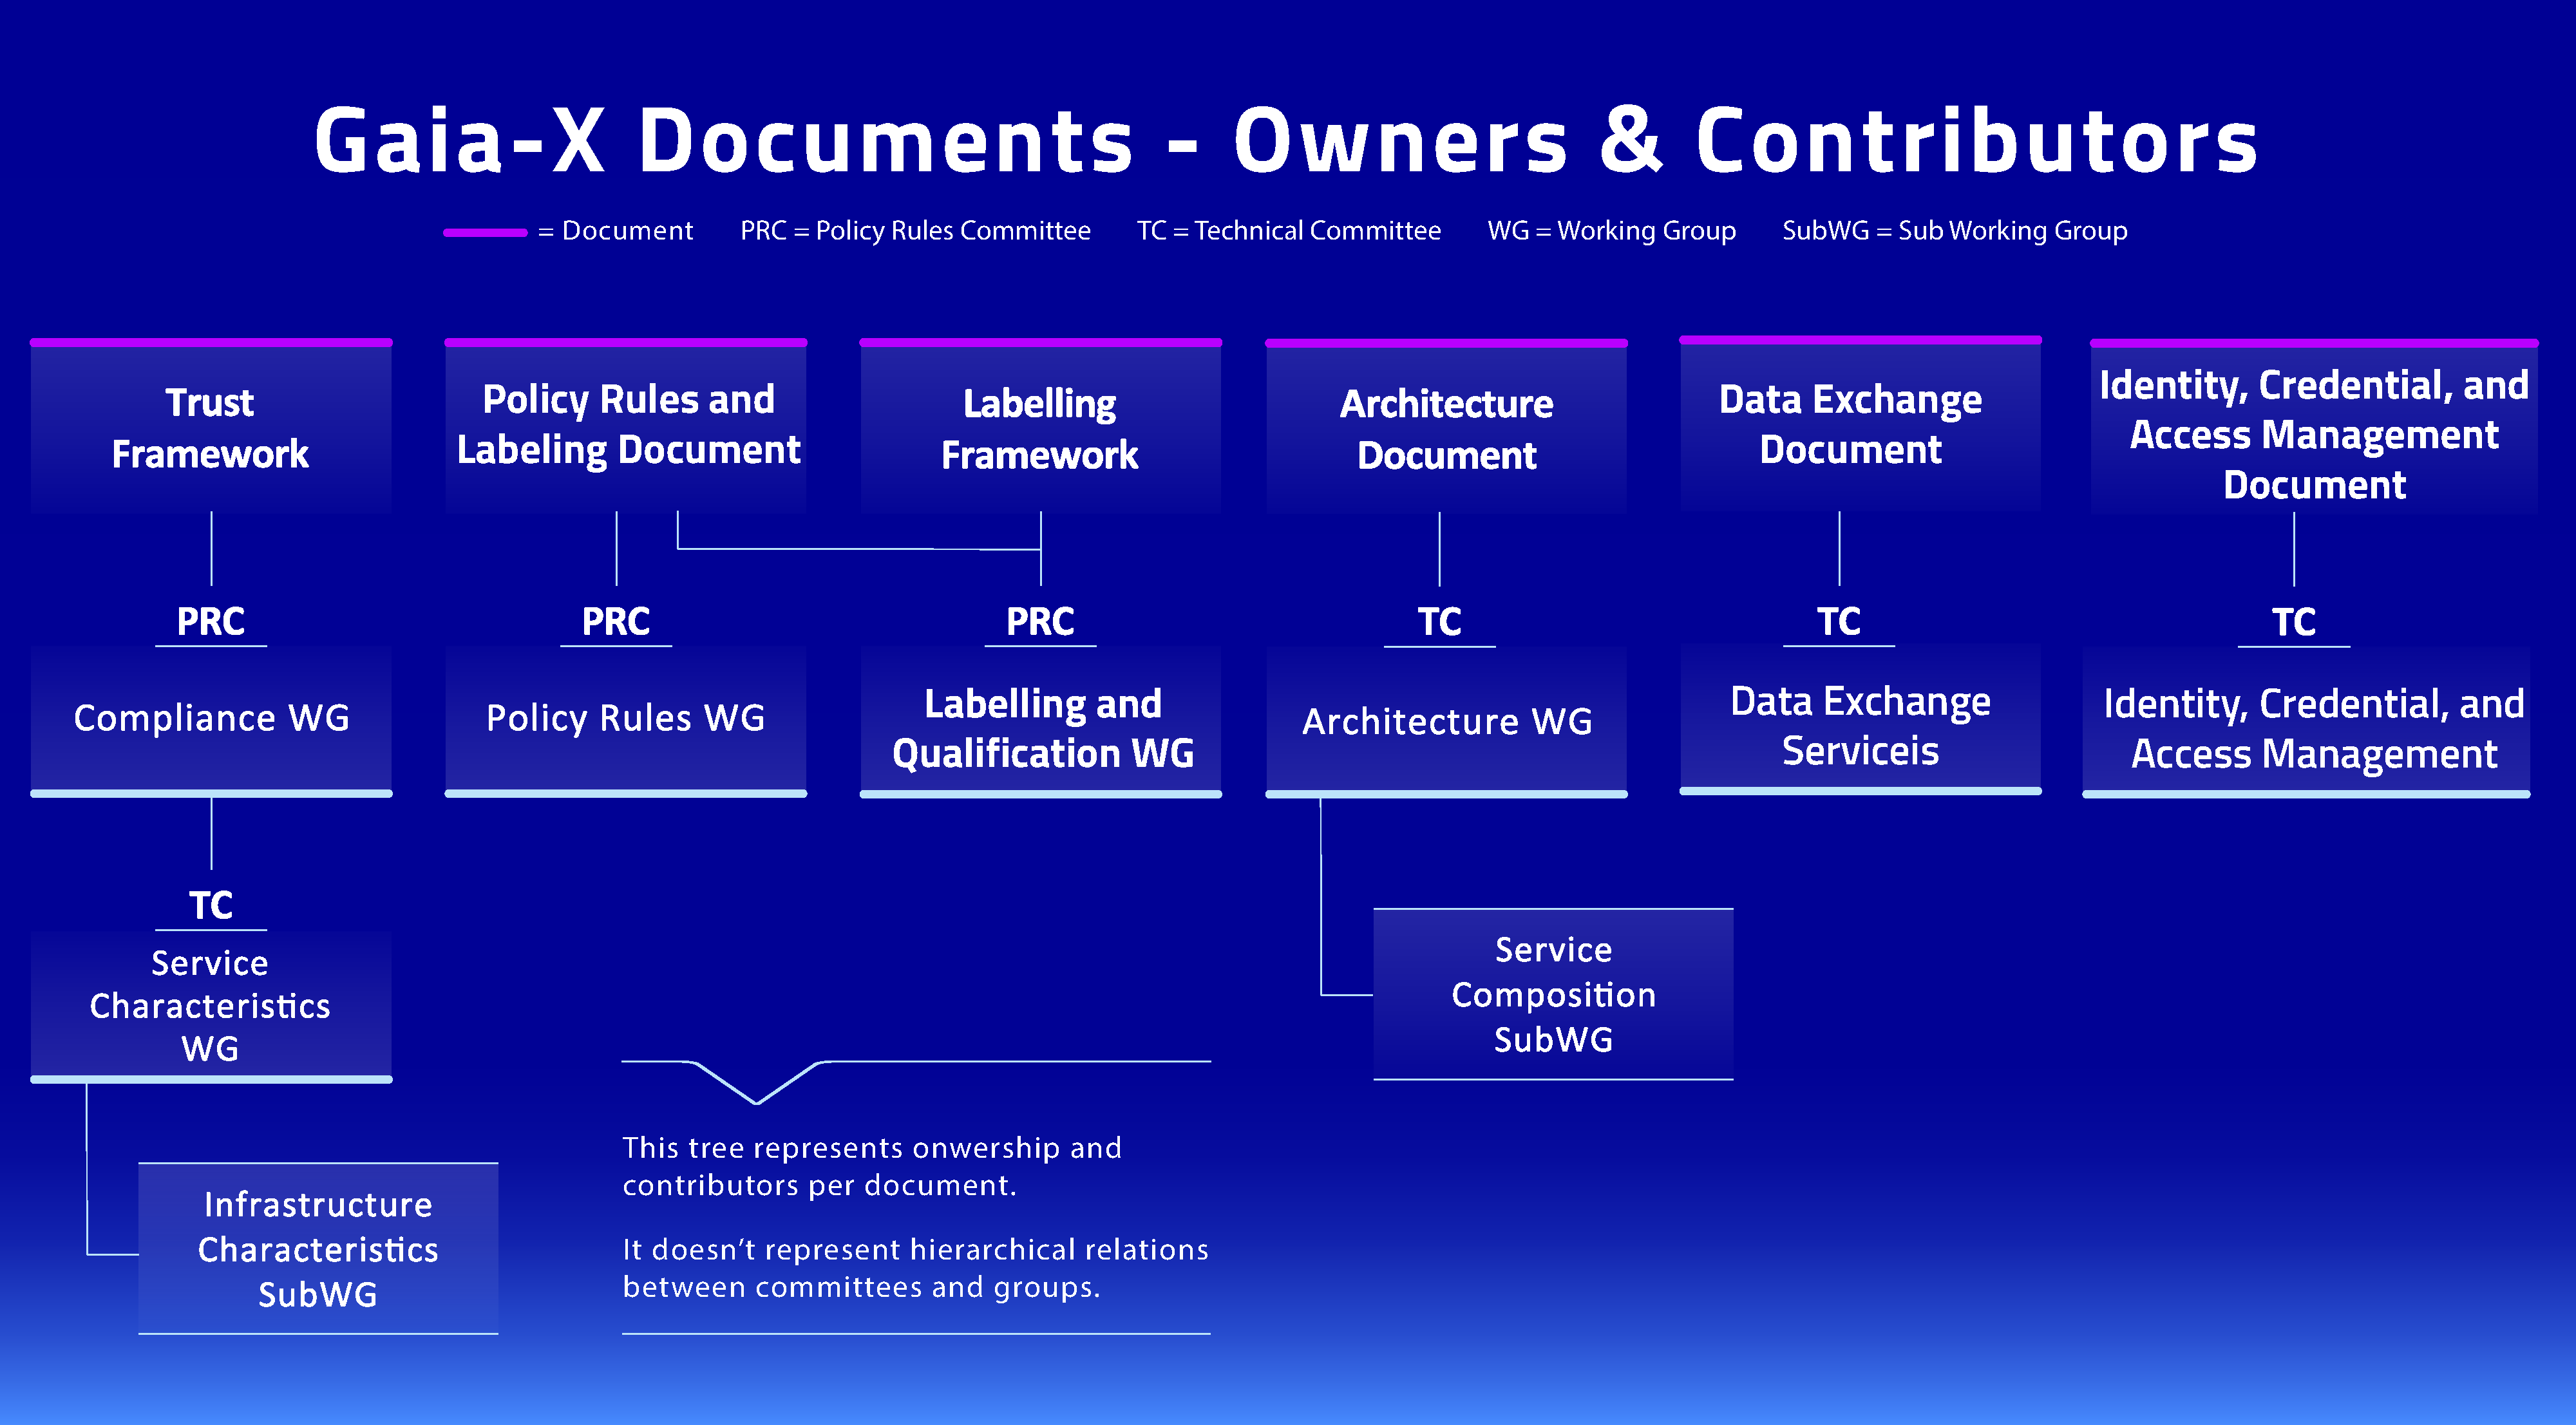
\includegraphics[width=\textwidth]{assets/committees-owners-and-contributors}
    \caption{~Gaia-X Documents - Owners \& Contributors~\cite{gaiax}}\label{fig:gaiax-documents-owners-and-contributors}
\end{figure}

% TODO: describe ecosystems and hubs

\section{Gaia-X Framework}\label{sec:gaia-x-framework}

These are categorized into three broad pillars: % this regards to Gaia-X framework (realization of goals)
\begin{itemize}
    \item Compliance:
    \item Federation:
    \item Data exchange:
\end{itemize}




% TODO: describe tthe trust framework

\clearpage


% Summary
%---------------------------------------------------------------

\chapter{Summary}\label{ch:summary}

A summary must be included in a master's thesis, as formulated in Section 34(6).





% APPENDIX
% these files should appear in the appendix of the thesis
% you can again use as many or as few files and chapters as required for your thesis
\appendix
% \include{contents/app-01-example}   % Glossar (\chapter{Glossar}  TEXT)
% \include{contents/app-02-example}   %
% \include{contents/app-03-example}   %

% Don't change these includes
%%%%%%%%%%%%%%%%%%%%%%%%%%%%%%%%%%%%%%%%%%%%%%%%%%%%%%%%%%%%%%%%%%%%%%%%%%
% Diese Datei nicht veraendern!
%%%%%%%%%%%%%%%%%%%%%%%%%%%%%%%%%%%%%%%%%%%%%%%%%%%%%%%%%%%%%%%%%%%%%%%%%%
\cleardoublepage
\phantomsection
\addcontentsline{toc}{chapter}{\listfigurename}
\listoffigures
 % List of Figures
%%%%%%%%%%%%%%%%%%%%%%%%%%%%%%%%%%%%%%%%%%%%%%%%%%%%%%%%%%%%%%%%%%%%%%%%%%
% Diese Datei nicht veraendern!
%%%%%%%%%%%%%%%%%%%%%%%%%%%%%%%%%%%%%%%%%%%%%%%%%%%%%%%%%%%%%%%%%%%%%%%%%%
\cleardoublepage
\phantomsection
\addcontentsline{toc}{chapter}{\listtablename}
\listoftables
 % List of Tables
%%%%%%%%%%%%%%%%%%%%%%%%%%%%%%%%%%%%%%%%%%%%%%%%%%%%%%%%%%%%%%%%%%%%%%%%%%
% Diese Datei nicht veraendern!
%%%%%%%%%%%%%%%%%%%%%%%%%%%%%%%%%%%%%%%%%%%%%%%%%%%%%%%%%%%%%%%%%%%%%%%%%%
\cleardoublepage
\phantomsection
\addcontentsline{toc}{chapter}{\bibname}
\printbibliography
 % Bibliography
\chapter{Acronyms}
\begin{acronym}
    \acro{GFXS}[GXFS]{Gaia-X Federation Services}
    \acro{P2P}[P2P]{Peer to Peer}
    \acro{WG}[WG]{Working Group}
    \acro{TC}[TC]{Technical Committee}
    \acro{GXFS}[GXFS]{Gaia-X Federation Services}
    \acro{IDS}[IDS]{International Data Spaces}
    \acro{PHS}[PHS]{Personal Health System}
    \acro{EHDS}[EHDS]{European Health Data Space}
    \acro{EU}[EU]{European Union}
    \acro{SME}[SME]{Small and medium-sized enterprise}
    \acro{IDSA}[IDSA]{International Data Spaces Association}
    \acro{IDS}[IDS]{International Data Spaces}
    \acro{IDS-RAM}[IDS-RAM]{International Data Spaces Reference Architecture Model}
    \acro{FL}[FL]{Federated Learning}
    \acro{MII}[MII]{Medical Informatics Initiative}
    \acro{OSDC}[OSDC]{Open Science Data Cloud}
    \acro{OCC}[OCC]{Open Commons Consortium}
    \acro{FDSM}[FDSM]{Foundation Data Space Models}
    \acro{GDPR}[GDPR]{General Data Protection Regulation}
    \acro{DTS}[DTS]{Digital Twin Space}
    \acro{DT}[DT]{Digital Twin}
    \acro{PLM}[PLM]{Product Lifecycle Management}
    \acro{EHR}[EHR]{Electronic Health Records}
    \acro{UDT}[UDT]{Urban Digital Twins}
\end{acronym}% TODO: sort alphabetically
 % Acronym definition and list of acronyms

\end{document}
